\section{Bohr Ra}\label{bohr-ra}

Tags: PC Creatore: Francesco C. Giocatore: Francesco Curcio Luogo: Azura
Razza: Gnomo Classe: Stregone Livello: 5

\section{Bohr Ra}\label{bohr-ra-1}

\begin{center}\rule{0.5\linewidth}{0.5pt}\end{center}

\begin{figure}
\centering
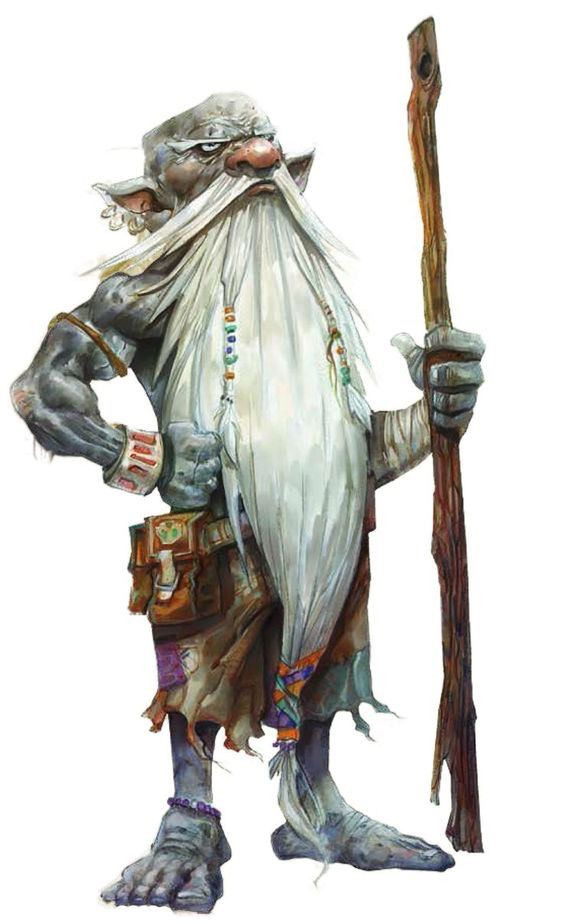
\includegraphics{2023-03-26_17.20.14.jpg}
\caption{2023-03-26 17.20.14.jpg}
\end{figure}

Informazioni Generali

Età:

Anno di nascita:

Paese di nascita:

Razza: Gnomo

Relazioni:

Alleati:

Nemesi:

Possedimenti importanti:

\begin{center}\rule{0.5\linewidth}{0.5pt}\end{center}

\subsection{1. Descrizione Generale}\label{descrizione-generale}

\begin{center}\rule{0.5\linewidth}{0.5pt}\end{center}

\begin{figure}
\centering
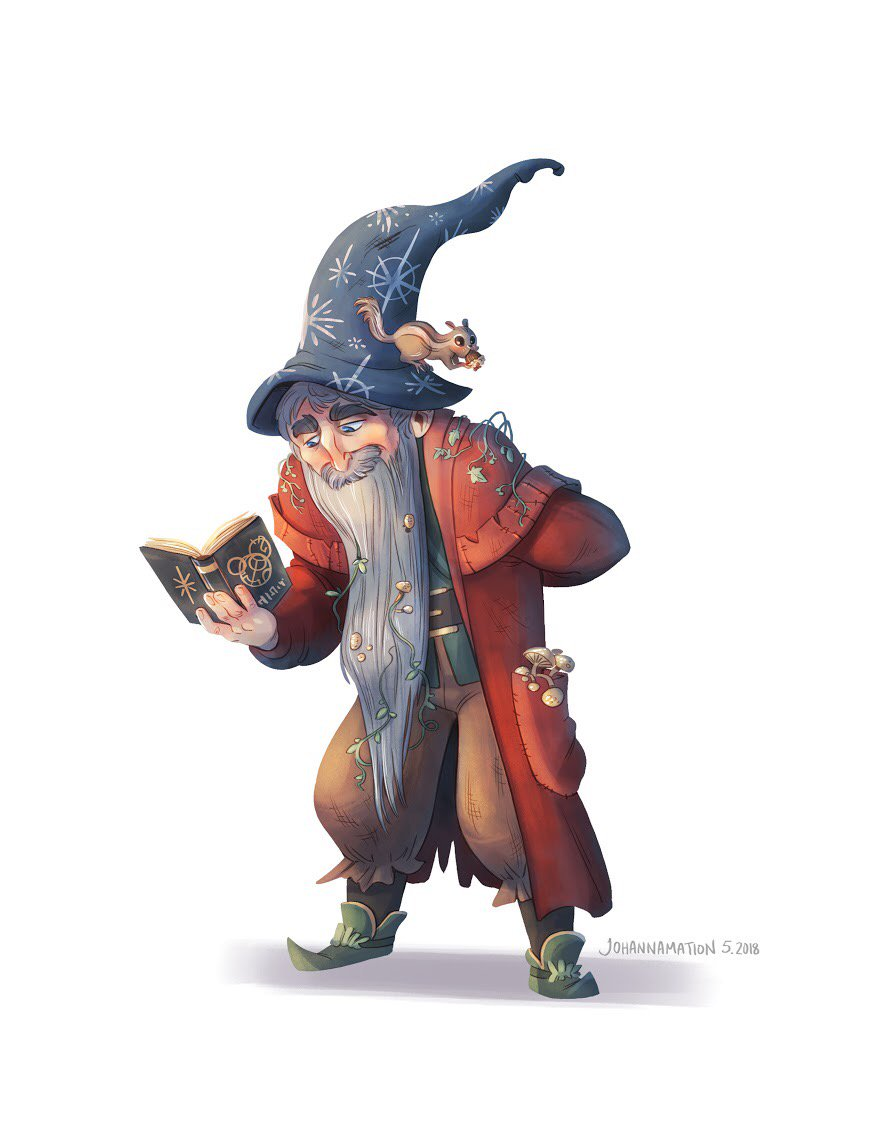
\includegraphics{DdXKFkiU8AYs_w2.jpg}
\caption{DdXKFkiU8AYs\_w2.jpg}
\end{figure}

Bohr Ra è un giovane gnomo di bassa statura e carnagione olivastra, con
capelli rossi arruffati e un paio di occhi velati dalle cataratte. A
causa della sua malattia, non riesce a vedere bene il mondo intorno a
lui, il che spesso lo rende goffo e maldestro. Nonostante questo, ha un
sorriso caldo e un atteggiamento curioso e allegro. Indossa vestiti
sobri ma ben curati, con un grembiule di pelle per proteggersi dalle
macchie di inchiostro durante i suoi studi.

\begin{quote}
``E se la magia è l'arte di manipolare la realtà, allora la necromanzia
è l'arte di manipolare la vita e la morte stesse.'' - Bohr Ra, il
giovane gnomo necromante.
\end{quote}

\subsection{2. Biografia}\label{biografia}

\begin{center}\rule{0.5\linewidth}{0.5pt}\end{center}

Bohr Ra è nato e cresciuto all'interno di una famiglia molto rispettata
all'interno del suo clan di gnomi. Fin dalla giovane età, ha mostrato un
grande interesse per la magia, passione che ha coltivato in segreto,
temendo il giudizio degli altri a causa della sua malattia. La
necromanzia è diventata la sua specializzazione preferita, non solo
perché gli ha permesso di esplorare le possibilità della vita e della
morte, ma anche perché crede che possa essere la chiave per curare la
sua malattia.

Dopo aver incontrato il vecchio necromante Brug Nas, Bohr Ra intraprese
ulteriori studi nelle arti arcane, durante i quali il suo maestro riuscì
a restituirgli la vista grazie ad un complesso rituale necromantico.
Grazie a questa guarigione, Bohr Ra poté finalmente vedere il mondo
intorno a lui con occhi nuovi e acuti, e questo gli permise di
approfondire ulteriormente la sua conoscenza della magia. La sua
determinazione nel voler trovare una cura per la sua malattia e il suo
talento innato per la necromanzia lo resero un discepolo prezioso per
Brug Nas, e la loro collaborazione portò a molte scoperte e innovazioni
nella pratica della necromanzia.

\subsection{3. Carriera}\label{carriera}

\begin{center}\rule{0.5\linewidth}{0.5pt}\end{center}

Nonostante la sua giovane età, Bohr Ra è già un mago molto promettente.
La sua grande scoperta è stata un misterioso libro degli incantesimi,
custodito in una sfera di metallo che si apre solo risolvendo intricati
rompicapi. Il libro contiene incantesimi estremamente potenti e
pericolosi, che Bohr Ra sta cercando di sbloccare risolvendo i
rompicapi. Tuttavia, finora è riuscito a risolvere solo i primi tre
livelli del rompicapo, e gli incantesimi che ha imparato da esso sono
ancora limitati. Inoltre, ha incontrato un vecchio necromante di nome
Brug Nas, che gli ha fatto da mentore e gli sta insegnando tutto ciò che
sa sulla necromanzia.

\subsection{4. Personalità}\label{personalituxe0}

\begin{center}\rule{0.5\linewidth}{0.5pt}\end{center}

Bohr Ra è una persona curiosa e appassionata, sempre alla ricerca di
nuovi incantesimi e modi per migliorare la sua magia. La sua
determinazione è spesso fonte di ispirazione per gli altri, ma a volte
può portarlo a compiere scelte discutibili. Ad esempio, ha deciso di
imparare un incantesimo di necromanzia che richiede l'uso di metodi
estremi e discutibili, come il prelievo di cadaveri di bambini o la
tortura di minoranze etniche. Nonostante tutto, Bohr Ra è una persona di
buon cuore, che cerca sempre di fare la cosa giusta e di proteggere
coloro che gli stanno a cuore.

\subsection{5. Coinvolgimenti in eventi
recenti}\label{coinvolgimenti-in-eventi-recenti}

\begin{center}\rule{0.5\linewidth}{0.5pt}\end{center}

\href{Untitled\%20Database\%205dd9b35a85b54745899bb10bc75cb6bf.csv}{Untitled
Database}

\subsection{6. Scheda personaggio}\label{scheda-personaggio}

\begin{center}\rule{0.5\linewidth}{0.5pt}\end{center}

\href{Info\%20PG\%208f526b9700b548eaac588929e340905c.csv}{Info PG}

\subsubsection{Statistiche e abilità}\label{statistiche-e-abilituxe0}

\begin{center}\rule{0.5\linewidth}{0.5pt}\end{center}

\href{Abilita\%CC\%80\%2082f8e70a09d245fe86b3ea906fa4405e.csv}{Abilità}

\subsubsection{Lista magie}\label{lista-magie}

\subsection{A. Descrizione originale}\label{a.-descrizione-originale}

\begin{center}\rule{0.5\linewidth}{0.5pt}\end{center}

Bohr Ra era un giovane gnomo che apparteneva ad una famiglia molto
rispettata nel suo clan. Fin dalla nascita, i suoi occhi erano sempre
stati velati dalle cataratte, una malattia che colpiva spesso i membri
della sua famiglia. Questa condizione gli impediva di vedere chiaramente
il mondo intorno a lui, e spesso lo rendeva oggetto di scherno e
derisione tra i suoi coetanei. Nonostante ciò, Bohr Ra era sempre stato
molto curioso e interessato alla magia. Trascorreva gran parte del suo
tempo libero a studiare gli incantesimi e a sperimentare con la magia,
sperando di trovare un modo per curare la sua malattia. Fu così che
scoprì la sua passione per la necromanzia, una forma di magia che gli
permise di imparare a manipolare la vita e la morte stesse. Mentre
studiava la necromanzia, Bohr Ra scoprì un misterioso libro degli
incantesimi fatto di una sfera di metallo che si apriva solo quando
risolto un intricato rompicapo. Questo libro era stato creato da un
potente necromante del passato, e conteneva incantesimi estremamente
potenti e pericolosi, che gli erano però preclusi. Inoltre il rompicapo
era composto da diversi livelli di difficoltà e sbloccandone di nuovi si
poteva accedere a incantesimi sempre più potenti. Fino ad ora Bohr è
riuscito a risolvere solo i primi 3 livelli del rompicapo (incantesimi
del terzo livello, 3 livelli eheh, come sono creativo). Poco tempo dopo,
il giovane gnomo incontrò un vecchio necromante che viveva in una
caverna isolata, Brug Nas. Il vecchio, che aveva una grande conoscenza
della necromanzia, riconobbe subito il talento di Bohr Ra e decise di
insegnargli tutto ciò che sapeva. Fu così che Bohr Ra intraprese
ulteriori studi nelle arti arcane, durante i quali il suo maestro riuscì
a restituirgli la vista grazie ad un complesso rituale~\st{che includeva
cadaveri di bambini, genocidi di massa e torture indicibili a minoranze
etniche}~necromantico.
